\section{Presentazione}

  \subsection{Presentazione Generale}
    Per il nostro sito è stato scelto come colore principale il blu. Abbiamo scelto questo colore perché spesso viene associato a sensazioni di stabilità e affidabilità, che il nostro sito vuole trasmettere. 
    Questi sono i colori che abbiamo associato al nostro colore principale:
    \begin{figure}[h]
      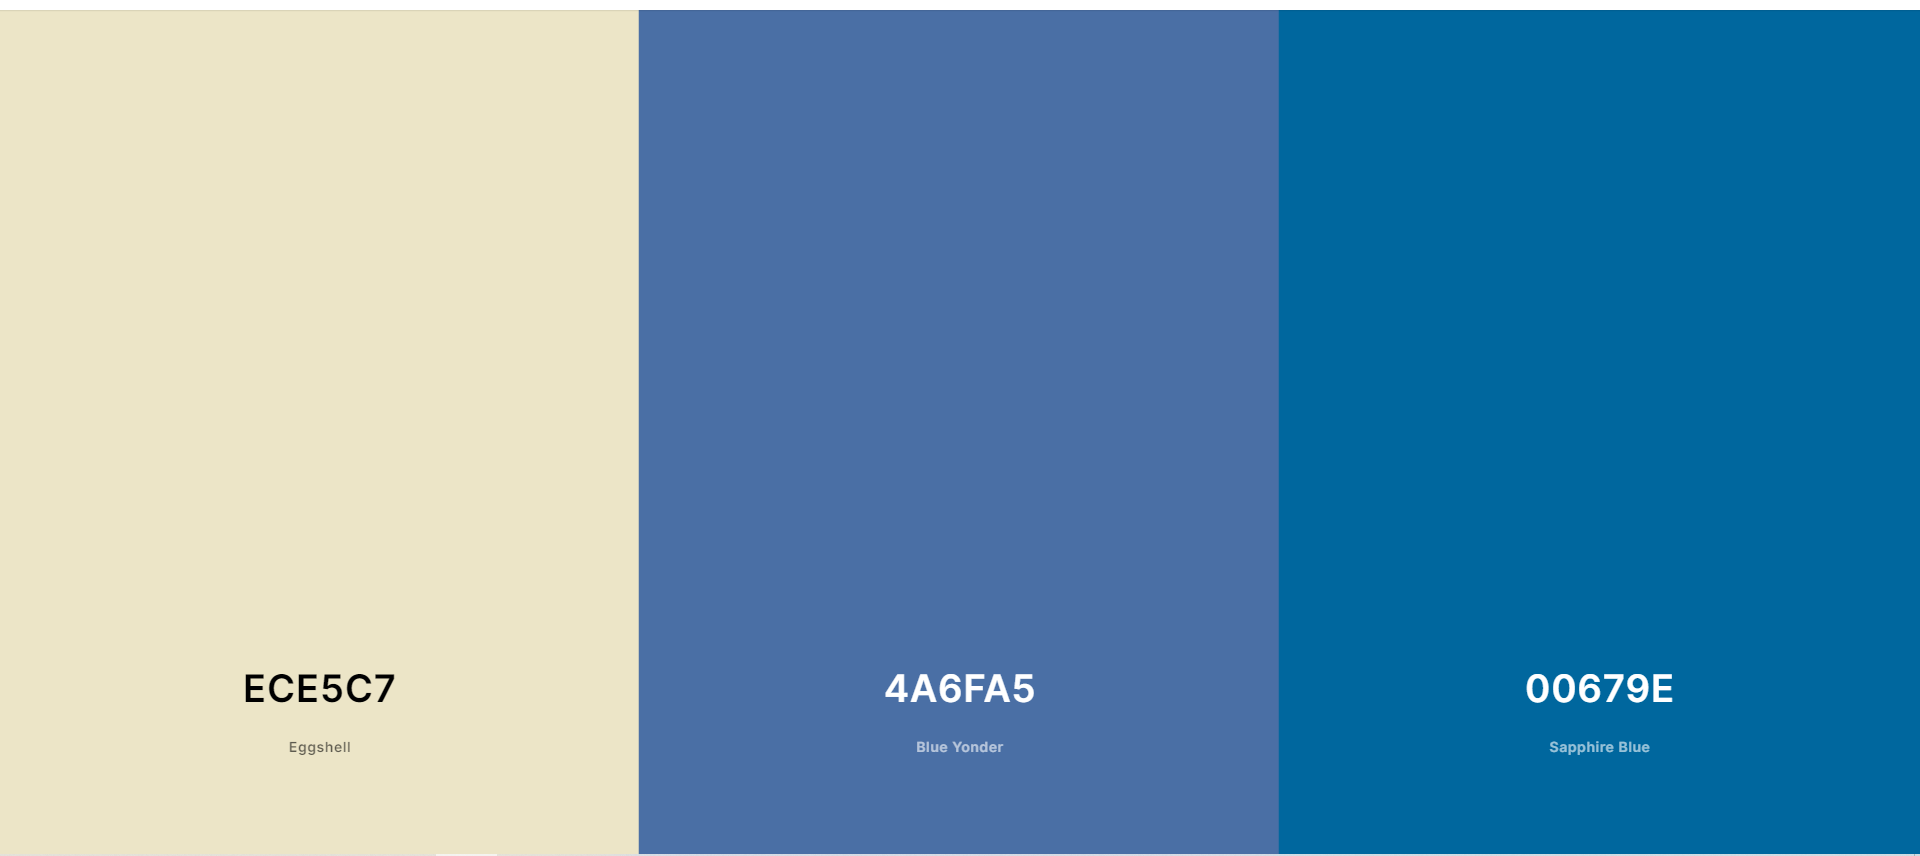
\includegraphics[scale=0.4]{Images/ColoriPaginaWeb.png}
      \centering
    \end{figure}

  \subsection{Desktop}
    Come dimensione massima per la versione desktop si è deciso di utilizzare 1024px, al fine di evitare difficoltà da parte dell'utente a visualizzare la pagina nella sua interezza. \\
    È presente un punto di rottura a 959px, al fine di migliorare la visibilità e le dimensioni di alcuni elementi.

  \subsection{Mobile}
    In modo simile alla versione Desktop, per la visualizzazione lato Mobile si è optato per punti di rottura; questi permettono di gestire al meglio la visualizzazione della pagina. \\
    Il principale punto di rottura per questa versione è a 694px. \\
    La visualizzazione Mobile differisce principalmente per alcuni elementi, quali:
    \begin{itemize}
      \item il footer viene rimpiazzato con l'header e viceversa. In questo modo, sarà più semplice per l'utente da mobile utilizzare i link dell'header che fungono come bottoni di un app;
      \item il logo viene rimosso;
      \item i contenuti che precedentemente venivano visualizzati di lato, ora vengono visualizzati in verticale per migliorare l'esperienza utente;
    \end{itemize}
  \subsection{Print}
    Per la funzionalità di stampa, ...